
\begin{frame}
    \frametitle{Inverse Fourier Transformation}
    \begin{columns}
        \begin{column}{80px}
            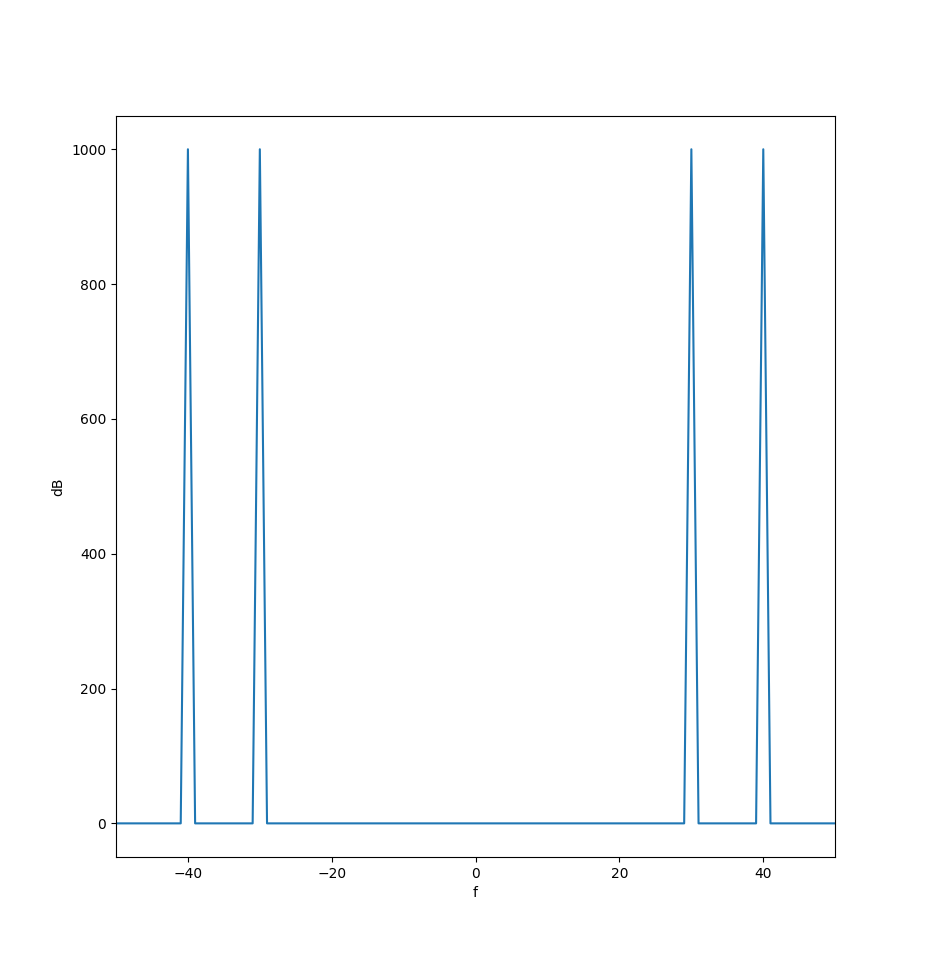
\includegraphics[width=80px, caption=Magnitude]{images/03-ift-mag.png} 
            \centering
            +
            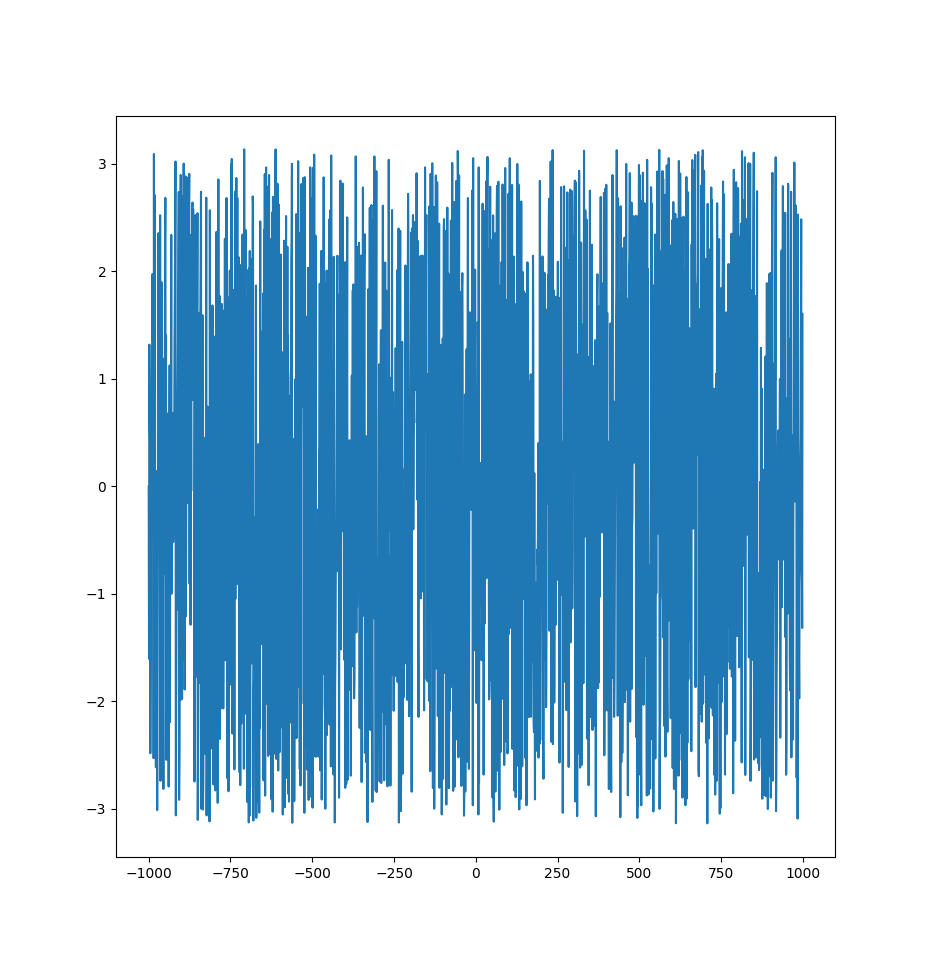
\includegraphics[width=80px]{images/03-ift-phase.png}
        \end{column}
        \hspace*{-40px}
        \begin{column}{5px}
            =
        \end{column}
        \hspace*{-40px}
        \begin{column}{100px}
            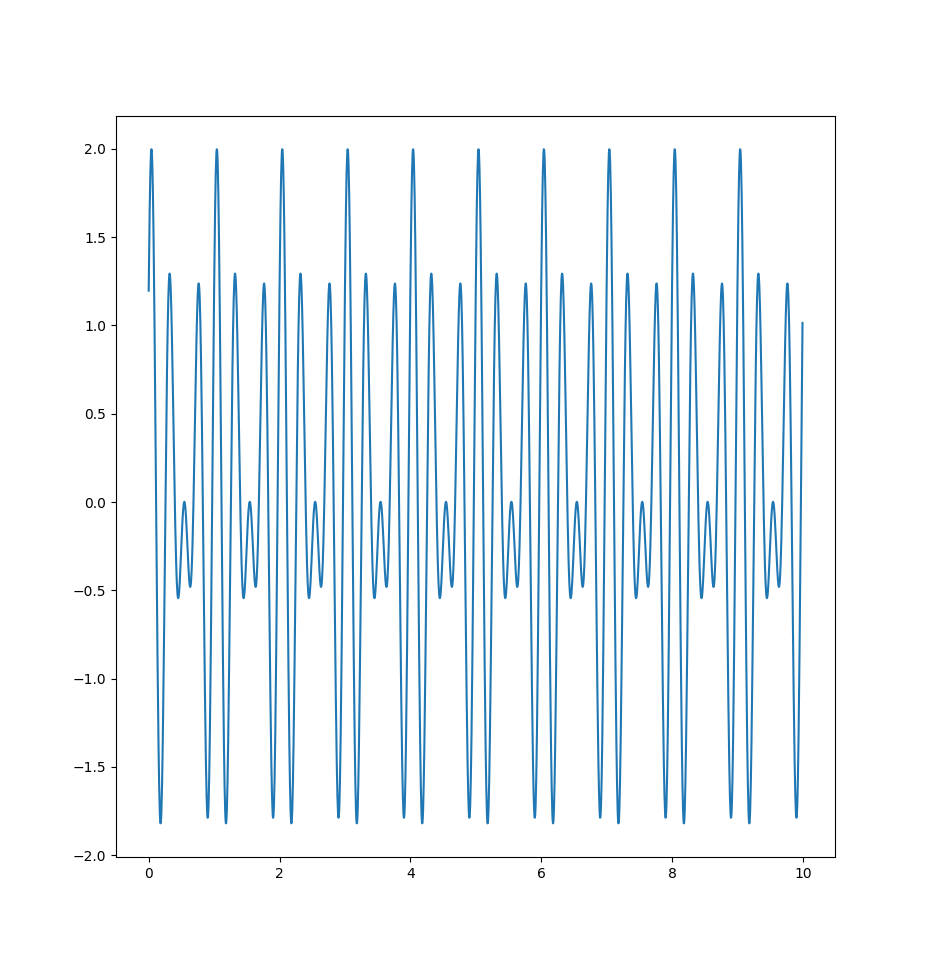
\includegraphics[width=100px]{images/03-ift-reconstructed.png} 
        \end{column}

    \end{columns}
\end{frame}

\begin{frame}
    \frametitle{Inverse Fourier Transformation}
    \begin{align*}
        g(t)=\int_{-\infty}^{\infty}{(\mathcal F g)(f)\cdot  e^{i2\pi f t}\ df}
    \end{align*} 
    \begin{itemize}
        \item Zwischen beiden Transformationen gehen keine Informationen verloren
    \end{itemize}
    \begin{align*}
        \Rightarrow \mathcal{F}^{-1}(\mathcal F g)(f)=g(x)
    \end{align*}
    \vspace*{-15px}
    \begin{itemize}
        \item[?] Wofür wird diese Rücktransformation benutzt
    \end{itemize}
\end{frame}

\begin{frame}
    \frametitle{Inverse Fourier Transformation}
    \begin{align*}
        g(t)=\int_{-\infty}^{\infty}{(\mathcal F g)(f)\cdot  e^{i2\pi f t}\ df}
    \end{align*} 
    \begin{itemize}
        \item Zwischen beiden Transformationen gehen keine Informationen verloren
    \end{itemize}
    \begin{align*}
        \Rightarrow \mathcal{F}^{-1}(\mathcal F g)(f)=g(x)
    \end{align*}
    \vspace*{-15px}
    \begin{itemize}
        \item Besonders nützlich z.B. für das Filtern von Frequenzen
    \end{itemize}
\end{frame}
